\documentclass[semifinal]{cpecmu}

%% This is a sample document demonstrating how to use the CPECMU
%% project template. If you are having trouble, see "cpecmu.pdf" for
%% documentation.

\projectNo{P069-1}
\acadyear{2024}

\titleTH{รายงานสหกิจศึกษา}
\titleEN{Cooperative Education Report}

\author{ณัฐพงษ์ เทพพิทักษ์}{Natthaphong Thepphithak}{640610634}
% \author{นายบรรจบ พบเอฟตลอด}{Banjob Pob-eftalord}{690610969}

\cpeadvisor{patiwet}
\cpecommittee{paskorn}
% \committee{รศ.ดร.\,นิพนธ์ ธีรอำพน}{Assoc.\,Prof.\,Nipon Theera-Umpon, Ph.D.}

%% Some possible packages to include:
\usepackage[final]{graphicx} % for including graphics

%% Add bookmarks and hyperlinks in the document.
\PassOptionsToPackage{hyphens}{url}
\usepackage[colorlinks=true,allcolors=Blue4,citecolor=red,linktoc=all]{hyperref}
\def\UrlLeft#1\UrlRight{$#1$}

%% Needed just by this example, but maybe not by most reports
\usepackage{afterpage} % for outputting
\usepackage{pdflscape} % for landscape figures and tables. 

%% Some other useful packages. Look these up to find out how to use
%% them.
% \usepackage{natbib}    % for author-year citation styles
% \usepackage{txfonts}
% \usepackage{appendix}  % for appendices on a per-chapter basis
% \usepackage{xtab}      % for tables that go over multiple pages
% \usepackage{subfigure} % for subfigures within a figure
% \usepackage{pstricks,pdftricks} % for access to special PostScript and PDF commands
% \usepackage{nomencl}   % if you have a list of abbreviations

%% if you're having problems with overfull boxes, you may need to increase
%% the tolerance to 9999
% \tolerance=9999

% \bibliographystyle{plain}
% \bibliographystyle{IEEEbib}
\bibliographystyle{IEEEtran}

% \renewcommand{\topfraction}{0.85}
% \renewcommand{\textfraction}{0.1}
% \renewcommand{\floatpagefraction}{0.75}

%% Example for glossary entry
%% Need to use glossary option
%% See glossaries package for complete documentation.
\ifglossary
  \newglossaryentry{lorem ipsum}{
    name=lorem ipsum,
    description={derived from Latin dolorem ipsum, translated as ``pain itself''}
  }
\fi

%% Uncomment this command to preview only specified LaTeX file(s)
%% imported with \include command below.
%% Any other file imported via \include but not specified here will not
%% be previewed.
%% Useful if your report is large, as you might not want to build
%% the entire file when editing a certain part of your report.
% \includeonly{chapters/intro,chapters/background}

\begin{document}
\maketitle
\makesignature

\ifproject
\begin{abstractTH}
% เขียนบทคัดย่อของรายงานที่นี่

% การเขียนรายงานเป็นส่วนหนึ่งของการทำรายงานวิศวกรรมคอมพิวเตอร์
% เพื่อทบทวนทฤษฎีที่เกี่ยวข้อง อธิบายขั้นตอนวิธีแก้ปัญหาเชิงวิศวกรรม และวิเคราะห์และสรุปผลการทดลองอุปกรณ์และระบบต่างๆ
% \enskip อย่างไรก็ดี การสร้างรูปเล่มรายงานให้ถูกรูปแบบนั้นเป็นขั้นตอนที่ยุ่งยาก
% แม้ว่าจะมีต้นแบบสำหรับใช้ในโปรแกรม Microsoft Word แล้วก็ตาม
% แต่นักศึกษาส่วนใหญ่ยังคงค้นพบว่าการใช้งานมีความซับซ้อน และเกิดความผิดพลาดในการจัดรูปแบบ กำหนดเลขหัวข้อ และสร้างสารบัญอยู่
% \enskip ภาควิชาวิศวกรรมคอมพิวเตอร์จึงได้จัดทำต้นแบบรูปเล่มรายงานโดยใช้ระบบจัดเตรียมเอกสาร
% \LaTeX{} เพื่อช่วยให้นักศึกษาเขียนรายงานได้อย่างสะดวกและรวดเร็วมากยิ่งขึ้น
รายงานนี้เป็นนำเสนอการสหกิจของวิศวกรรมศาสตรสาขาคอมพิวเตอร์ในตำแหน่ง DevOps Engineer 
ที่ SCB TechX ซึ่งเป็นส่วนหนึ่งของธนาคารไทยพาณิชย์ (SCB) 
ในระหว่างช่วงเวลาของการทำงาน ได้มีส่วนร่วมในการสนับสนุนทีมพัฒนาซอฟต์แวร์ โดยเฉพาะในด้านการสร้างและการลบทรัพยากร 
รวมถึงการพัฒนาและบำรุงรักษา Terraform Modules สำหรับโมดูลกลางที่ถูกใช้งานทั้งใน SCB TechX และ SCB ซึ่งทั้งหมดนี้เป็นส่วนสำคัญในการเพิ่มประสิทธิภาพและความคล่องตัวให้กับกระบวนการ DevOps ของ
บริษัท เพื่อตอบสนองความต้องการของลูกค้าอย่างมีประสิทธิภาพและรวดเร็ว
\end{abstractTH}

\begin{abstract}
This report presents a cooperative education experience in Computer Engineering for the position of DevOps Engineer at SCB TechX, a subsidiary of Siam Commercial Bank (SCB). 
During the work period, I participated in supporting the software development team, particularly in the creation and deletion of resources, as well as the development and maintenance of Terraform Modules for central modules used in both SCB TechX and SCB. 
All of these activities were crucial in enhancing the efficiency and agility of the company's DevOps processes to effectively and rapidly meet customer needs.
\end{abstract}

\iffalse
\begin{dedication}
This document is dedicated to all Chiang Mai University students.

Dedication page is optional.
\end{dedication}
\fi % \iffalse

\begin{acknowledgments}
    การที่ข้าพเจ้าได้มาปฏิบัติงานสหกิจศึกษา ณ บริษัท เอสซีบี เทคเอกซ์ จำกัด  ตั้งแต่วันที่ 4 มิถุนายน 2567  ถึง วันที่  25 ตุลาคม 2567  ส่งผลให้ข้าพเจ้าได้รับความรู้และประสบการณ์ต่างๆ ที่มีค่ามากมาย สำหรับรายงานวิชาสหกิจศึกษาฉบับนี้  สำเร็จลงได้ด้วยดีจากความร่วมมือและสนับสนุนจากหลายฝ่าย  ดังนี้
    \begin{enumerate}
        \item พีรวัตร อยู่ใจเย็น ตำแหน่ง Sernior DevOps Engineer
        \item ภัทรพล หมวกมณี ตำแหน่ง DevOps Engineer
    \end{enumerate}
    และบุคคลท่านอื่นๆที่ไม่ได้กล่าวนามทุกท่านที่ได้ให้คำแนะนำช่วยเหลือในการจัดทำรายงาน
	ข้าพเจ้าใคร่ขอขอบพระคุณผู้ที่มีส่วนเกี่ยวข้องทุกท่าน ที่มีส่วนร่วมในการให้ข้อมูล เป็นที่ปรึกษาในการทำรายงานฉบับนี้จนเสร็จสมบูรณ์ ตลอดจนให้การดูแลและให้ความเข้าใจเกี่ยวกับชีวิตของการทำงานจริง ข้าพเจ้าขอขอบคุณ ไว้ ณ ที่นี้
    \acksign{2024}{10}{25}
\end{acknowledgments}%
\fi % \ifproject

\contentspage % generate the table of contents

\ifproject
\tablelistpage
\figurelistpage

% \tablelistpage
\fi % \ifproject

% \abbrlist % this page is optional

% \symlist % this page is optional

% \preface % this section is optional


\pagestyle{empty}\cleardoublepage
\normalspacing \setcounter{page}{1} \pagenumbering{arabic} \pagestyle{cpecmu}

\chapter{\ifenglish Introduction\else ข้อมูลทั่วไปของบรษัท\fi}

\section{\ifenglish Company History\else ประวัติความเป็นมาของบริษัท\fi}

SCB TechX \cite{techxWebsite} ก่อตั้งขึ้นจากความร่วมมือระหว่าง SCBX กลุ่มธุรกิจการเงินและเทคโนโลยีชั้นนำของไทย และ Publicis Sapient บริษัทที่ปรึกษาด้านดิจิทัลทรานส์ฟอร์เมชันระดับโลก มีจุดมุ่งหมายเพื่อมอบบริการด้านเทคโนโลยีที่ตอบสนองความต้องการของธุรกิจต่าง ๆ ตั้งแต่การสร้างนวัตกรรมและผลิตภัณฑ์ใหม่ ไปจนถึงการนำเทคโนโลยีมาเพิ่มประสิทธิภาพในการดำเนินงาน

บริษัทมีความเชี่ยวชาญในการพัฒนาโซลูชันในระดับองค์กร (Enterprise-grade solutions) ที่ปลอดภัยและรองรับการใช้งานของฐานลูกค้าจำนวนมาก นอกจากนี้ SCB TechX ยังจัดองค์กรในรูปแบบ Startup เพื่อลดความซ้ำซ้อนในการทำงานและส่งเสริมความคิดริเริ่มใหม่ ๆ ทำให้สามารถพัฒนาโซลูชันให้กับลูกค้าได้อย่างรวดเร็วและมีประสิทธิภาพ


\section{\ifenglish Company Product\else บริการและผลิตภัณฑ์ของบริษัท\fi}
SCB TechX นำเสนอนวัตกรรมที่พร้อมใช้งานหลากหลายด้าน \cite{techxProduct} ทั้งระบบยืนยันตัวตนแบบดิจิทัลด้วยระบบ KYC \cite{whatIsKYC} ซึ่งทางบริษัทจะเรียกว่า eKYC และแพลตฟอร์มทางการเงินที่หลากหลาย นวัตกรรมเหล่านี้สามารถเชื่อมต่อกับระบบของลูกค้าได้อย่างรวดเร็วและง่ายดาย พร้อมทั้งปรับแต่งตามความต้องการเฉพาะของธุรกิจ ส่งผลให้ลูกค้าของ SCB TechX สามารถเปิดตัวบริการใหม่หรือยกระดับการให้บริการได้อย่างทันท่วงที

นอกจากนี้ SCB TechX ยังให้บริการที่ครอบคลุมด้านการให้คำปรึกษาทางเทคโนโลยี (Technology Consulting), โซลูชันด้านโครงสร้างพื้นฐานและแพลตฟอร์ม (Infrastructure \& Platforms), โซลูชันคลาวด์ (Cloud Solutions), แพลตฟอร์มเทคโนโลยีแบบครบวงจร (xPlatform), การจัดการข้อมูลและความปลอดภัย (Data \& Security), และโซลูชันด้านข้อมูลและ AI (TechX Data \& AI Solutions) ที่ออกแบบมาเพื่อรองรับและเสริมสร้างศักยภาพให้กับธุรกิจในยุคดิจิทัล

\clearpage

\section{\ifenglish Organization\else ผู้บริหารของบริษัท\fi}
\begin{figure}[ht]
    \begin{center}
    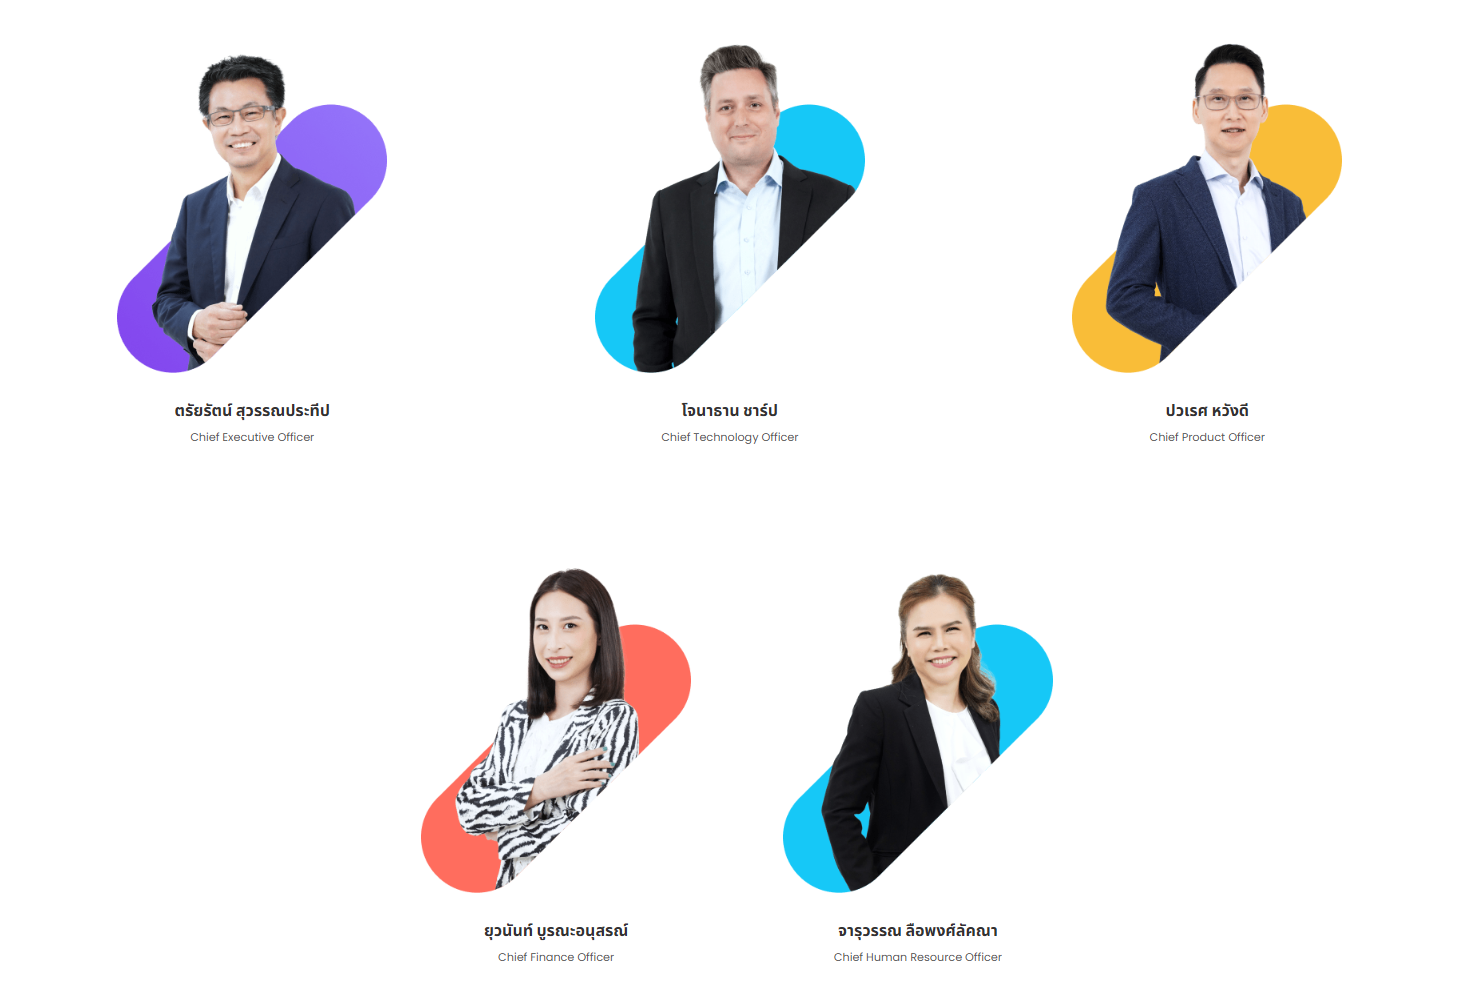
\includegraphics[scale=0.3]{images/org.png}
    \end{center}
    \caption[Board Of Director]{ผู้บริหารและตำแหน่งของบริษัท}
    \label{fig:org}
\end{figure}

% \section{\ifenglish Objectives\else วัตถุประสงค์ของโครงงาน\fi}
% \begin{enumerate}
%     \item
% \end{enumerate}

% \section{\ifenglish Project scope\else ขอบเขตของโครงงาน\fi}

% \subsection{\ifenglish Hardware scope\else ขอบเขตด้านฮาร์ดแวร์\fi}

% \subsection{\ifenglish Software scope\else ขอบเขตด้านซอฟต์แวร์\fi}

% \section{\ifenglish Expected outcomes\else ประโยชน์ที่ได้รับ\fi}

% \section{\ifenglish Technology and tools\else เทคโนโลยีและเครื่องมือที่ใช้\fi}

% \subsection{\ifenglish Hardware technology\else เทคโนโลยีด้านฮาร์ดแวร์\fi}

% \subsection{\ifenglish Software technology\else เทคโนโลยีด้านซอฟต์แวร์\fi}

% \section{\ifenglish Project plan\else แผนการดำเนินงาน\fi}

% \begin{plan}{6}{2020}{2}{2021}
%     \planitem{7}{2020}{8}{2020}{ศึกษาค้นคว้า}
%     \planitem{8}{2020}{1}{2021}{ชิล}
%     \planitem{2}{2021}{2}{2021}{เผา}
%     \planitem{12}{2019}{1}{2022}{ทดสอบ}
% \end{plan}

% \section{\ifenglish Roles and responsibilities\else บทบาทและความรับผิดชอบ\fi}
% อธิบายว่าในการทำงาน นศ. มีการกำหนดบทบาทและแบ่งหน้าที่งานอย่างไรในการทำงาน จำเป็นต้องใช้ความรู้ใดในการทำงานบ้าง

% \section{\ifenglish%
% Impacts of this project on society, health, safety, legal, and cultural issues
% \else%
% ผลกระทบด้านสังคม สุขภาพ ความปลอดภัย กฎหมาย และวัฒนธรรม
% \fi}

% แนวทางและโยชน์ในการประยุกต์ใช้งานโครงงานกับงานในด้านอื่นๆ รวมถึงผลกระทบในด้านสังคมและสิ่งแวดล้อมจากการใช้ความรู้ทางวิศวกรรมที่ได้

% \chapter{\ifenglish Background Knowledge and Theory\else ทฤษฎีที่เกี่ยวข้อง\fi}

การทำโครงงาน เริ่มต้นด้วยการศึกษาค้นคว้า ทฤษฎีที่เกี่ยวข้อง หรือ งานวิจัย/โครงงาน ที่เคยมีผู้นำเสนอไว้แล้ว ซึ่งเนื้อหาในบทนี้ก็จะเกี่ยวกับการอธิบายถึงสิ่งที่เกี่ยวข้องกับโครงงาน เพื่อให้ผู้อ่านเข้าใจเนื้อหาในบทถัด ๆ ไปได้ง่ายขึ้น

\section{The first section}
The text for Section 1 goes here.

\section{Second section}
Section 2 text.

\subsection{Subsection heading goes here}

Subsection 1 text

\subsubsection{Subsubsection 1 heading goes here}
Subsubsection 1 text

\subsubsection{Subsubsection 2 heading goes here}
Subsubsection 2 text

\section{Third section}
Section 3 text. The dielectric constant\index{dielectric constant}
at the air-metal interface determines
the resonance shift\index{resonance shift} as absorption or capture occurs
is shown in Equation~\eqref{eq:dielectric}:

\begin{equation}\label{eq:dielectric}
k_1=\frac{\omega}{c({1/\varepsilon_m + 1/\varepsilon_i})^{1/2}}=k_2=\frac{\omega
\sin(\theta)\varepsilon_\mathit{air}^{1/2}}{c}
\end{equation}

\noindent
where $\omega$ is the frequency of the plasmon, $c$ is the speed of
light, $\varepsilon_m$ is the dielectric constant of the metal,
$\varepsilon_i$ is the dielectric constant of neighboring insulator,
and $\varepsilon_\mathit{air}$ is the dielectric constant of air.

\section{About using figures in your report}

% define a command that produces some filler text, the lorem ipsum.
\newcommand{\loremipsum}{
  \textit{Lorem ipsum dolor sit amet, consectetur adipisicing elit, sed do
  eiusmod tempor incididunt ut labore et dolore magna aliqua. Ut enim ad
  minim veniam, quis nostrud exercitation ullamco laboris nisi ut
  aliquip ex ea commodo consequat. Duis aute irure dolor in
  reprehenderit in voluptate velit esse cillum dolore eu fugiat nulla
  pariatur. Excepteur sint occaecat cupidatat non proident, sunt in
  culpa qui officia deserunt mollit anim id est laborum.}\par}

\begin{figure}
  \centering

  \fbox{
     \parbox{.6\textwidth}{\loremipsum}
  }

  % To include an image in the figure, say myimage.pdf, you could use
  % the following code. Look up the documentation for the package
  % graphicx for more information.
  % \includegraphics[width=\textwidth]{myimage}

  \caption[Sample figure]{This figure is a sample containing \gls{lorem ipsum},
  showing you how you can include figures and glossary in your report.
  You can specify a shorter caption that will appear in the List of Figures.}
  \label{fig:sample-figure}
\end{figure}

Using \verb.\label. and \verb.\ref. commands allows us to refer to
figures easily. If we can refer to Figures
\ref{fig:walrus} and \ref{fig:sample-figure} by name in the {\LaTeX}
source code, then we will not need to update the code that refers to it
even if the placement or ordering of the figures changes.

\loremipsum\loremipsum

% This code demonstrates how to get a landscape table or figure. It
% uses the package lscape to turn everything but the page number into
% landscape orientation. Everything should be included within an
% \afterpage{ .... } to avoid causing a page break too early.
\afterpage{
  \begin{landscape}
  \begin{table}
    \caption{Sample landscape table}
    \label{tab:sample-table}

    \centering

    \begin{tabular}{c||c|c}
        Year & A & B \\
        \hline\hline
        1989 & 12 & 23 \\
        1990 & 4 & 9 \\
        1991 & 3 & 6 \\
    \end{tabular}
  \end{table}
  \end{landscape}
}

\loremipsum\loremipsum\loremipsum

\section{Overfull hbox}

When the \verb.semifinal. option is passed to the \verb.cpecmu. document class,
any line that is longer than the line width, i.e., an overfull hbox, will be
highlighted with a black solid rule:
\begin{center}
\begin{minipage}{2em}
juxtaposition
\end{minipage}
\end{center}

\section{\ifenglish%
\ifcpe CPE \else ISNE \fi knowledge used, applied, or integrated in this project
\else%
ความรู้ตามหลักสูตรซึ่งถูกนำมาใช้หรือบูรณาการในโครงงาน
\fi
}

อธิบายถึงความรู้ และแนวทางการนำความรู้ต่าง ๆ ที่ได้เรียนตามหลักสูตร ซึ่งถูกนำมาใช้ในโครงงาน

\section{\ifenglish%
Extracurricular knowledge used, applied, or integrated in this project
\else%
ความรู้นอกหลักสูตรซึ่งถูกนำมาใช้หรือบูรณาการในโครงงาน
\fi
}

อธิบายถึงความรู้ต่าง ๆ ที่เรียนรู้ด้วยตนเอง และแนวทางการนำความรู้เหล่านั้นมาใช้ในโครงงาน

% \chapter{\ifproject%
\ifenglish Project Structure and Methodology\else โครงสร้างและขั้นตอนการทำงาน\fi
\else%
\ifenglish Project Structure\else โครงสร้างของรายงาน\fi
\fi
}

ในบทนี้จะกล่าวถึงหลักการ และการออกแบบระบบ

\makeatletter

% \renewcommand\section{\@startsection {section}{1}{\z@}%
%                                    {13.5ex \@plus -1ex \@minus -.2ex}%
%                                    {2.3ex \@plus.2ex}%
%                                    {\normalfont\large\bfseries}}

\makeatother
%\vspace{2ex}
% \titleformat{\section}{\normalfont\bfseries}{\thesection}{1em}{}
% \titlespacing*{\section}{0pt}{10ex}{0pt}

\section{Alice in Wonderland}

\begin{figure}
\begin{center}
\includegraphics{800px-Briny_Beach.jpg}
\end{center}
\caption[Poem]{The Walrus and the Carpenter}
\label{fig:walrus}
\end{figure}

\subsection{The Black Kitten}
  One thing was certain, that the WHITE kitten had had nothing to
do with it:---it was the black kitten's fault entirely~\cite{aiw}.  For the
white kitten had been having its face washed by the old cat for
the last quarter of an hour (and bearing it pretty well,
considering); so you see that it COULDN'T have had any hand in
the mischief.

  The way Dinah washed her children's faces was this:  first she
held the poor thing down by its ear with one paw, and then with
the other paw she rubbed its face all over, the wrong way,
beginning at the nose:  and just now, as I said, she was hard at
work on the white kitten, which was lying quite still and trying
to purr---no doubt feeling that it was all meant for its good.

  But the black kitten had been finished with earlier in the
afternoon, and so, while Alice was sitting curled up in a corner
of the great arm-chair, half talking to herself and half asleep,
the kitten had been having a grand game of romps with the ball of
worsted Alice had been trying to wind up, and had been rolling it
up and down till it had all come undone again; and there it was,
spread over the hearth-rug, all knots and tangles, with the
kitten running after its own tail in the middle.

\subsection{The Reproach}

  `Oh, you wicked little thing!' cried Alice, catching up the
kitten, and giving it a little kiss to make it understand that it
was in disgrace.  `Really, Dinah ought to have taught you better
manners!  You OUGHT, Dinah, you know you ought!' she added,
looking reproachfully at the old cat, and speaking in as cross a
voice as she could manage---and then she scrambled back into the
arm-chair, taking the kitten and the worsted with her, and began
winding up the ball again.  But she didn't get on very fast, as
she was talking all the time, sometimes to the kitten, and
sometimes to herself.  Kitty sat very demurely on her knee,
pretending to watch the progress of the winding, and now and then
putting out one paw and gently touching the ball, as if it would
be glad to help, if it might.

  `Do you know what to-morrow is, Kitty?' Alice began.  `You'd
have guessed if you'd been up in the window with me---only Dinah
was making you tidy, so you couldn't.  I was watching the boys
getting in stick for the bonfire---and it wants plenty of
sticks, Kitty!  Only it got so cold, and it snowed so, they had
to leave off.  Never mind, Kitty, we'll go and see the bonfire
to-morrow.'  Here Alice wound two or three turns of the worsted
round the kitten's neck, just to see how it would look:  this led
to a scramble, in which the ball rolled down upon the floor, and
yards and yards of it got unwound again.

  `Do you know, I was so angry, Kitty,' Alice went on as soon as
they were comfortably settled again, `when I saw all the mischief
you had been doing, I was very nearly opening the window, and
putting you out into the snow!  And you'd have deserved it, you
little mischievous darling!  What have you got to say for
yourself?  Now don't interrupt me!' she went on, holding up one
finger.  `I'm going to tell you all your faults.  Number one:
you squeaked twice while Dinah was washing your face this
morning.  Now you can't deny it, Kitty:  I heard you!  What that
you say?' (pretending that the kitten was speaking.)  `Her paw
went into your eye?  Well, that's YOUR fault, for keeping your
eyes open---if you'd shut them tight up, it wouldn't have
happened.  Now don't make any more excuses, but listen!  Number
two:  you pulled Snowdrop away by the tail just as I had put down
the saucer of milk before her!  What, you were thirsty, were you?

% \chapter{\ifproject%
\ifenglish Experimentation and Results\else การทดลองและผลลัพธ์\fi
\else%
\ifenglish System Evaluation\else การประเมินระบบ\fi
\fi}

ในบทนี้จะทดสอบเกี่ยวกับการทำงานในฟังก์ชันหลัก ๆ

\ifproject
% \chapter{\ifenglish Conclusions and Discussions\else บทสรุปและข้อเสนอแนะ\fi}

\section{\ifenglish Conclusions\else สรุปผล\fi}

นศ. ควรสรุปถึงข้อจำกัดของระบบในด้านต่าง ๆ ที่ระบบมีในเนื้อหาส่วนนี้ด้วย

\section{\ifenglish Challenges\else ปัญหาที่พบและแนวทางการแก้ไข\fi}

ในการทำโครงงานนี้ พบว่าเกิดปัญหาหลัก ๆ ดังนี้

\section{\ifenglish%
Suggestions and further improvements
\else%
ข้อเสนอแนะและแนวทางการพัฒนาต่อ
\fi
}

ข้อเสนอแนะเพื่อพัฒนาโครงงานนี้ต่อไป มีดังนี้

\fi

\bibliography{sampleReport}

\ifproject
\normalspacing
\appendix
\chapter{เอกสารสำคัญที่เกี่ยวข้อง}
\begin{itemize}
    \item \textbf{เอกสารสำคัญของคณะ}
          \begin{itemize}
              \item \hyperlink{target:03-04}{วศ.สก.-03/04 รายงานตัวเข้าสหกิจศึกษา} (หน้า \pageref{page:03-04})
              \item \hyperlink{target:03}{วศ.ฝ.ค-03 แบบฟอร์มยืนยันการรับนักศึกษา} (หน้า \pageref{page:03})
              \item \hyperlink{target:11}{วศ.สก.-11 แบบสรุปผลการปฏิบัติงานสหกิจศึกษา} (หน้า \pageref{page:11})
          \end{itemize}
    \item \textbf{เอกสารสำคัญที่เกี่ยวข้องกับงาน}
          \begin{itemize}
              \item \hyperlink{target:docker}{เอกสารสรุปสิ่งที่ได้เรียนรู้และลองทำ Docker} (หน้า \pageref{page:docker})
              \item \hyperlink{target:kube}{เอกสารสรุปสิ่งที่ได้เรียนรู้และลองทำ Kubernetes} (หน้า \pageref{page:kube})
              \item \hyperlink{target:jenkins}{เอกสารสรุปสิ่งที่ได้เรียนรู้และลองทำ Jenkins} (หน้า \pageref{page:jenkins})
              \item \hyperlink{target:terraform}{เอกสารสรุปสิ่งที่ได้เรียนรู้และลองทำ Terraform} (หน้า \pageref{page:terraform})
              \item \hyperlink{target:monitoring}{เอกสารสรุปสิ่งที่ได้เรียนรู้เกี่ยวกับ Monitoring Tools} (หน้า \pageref{page:monitoring})
              \item \hyperlink{target:elk}{เอกสารสรุปสิ่งที่ได้เรียนรู้เกี่ยวกับ ELK Stack} (หน้า \pageref{page:elk})
          \end{itemize}
\end{itemize}

% คณะ
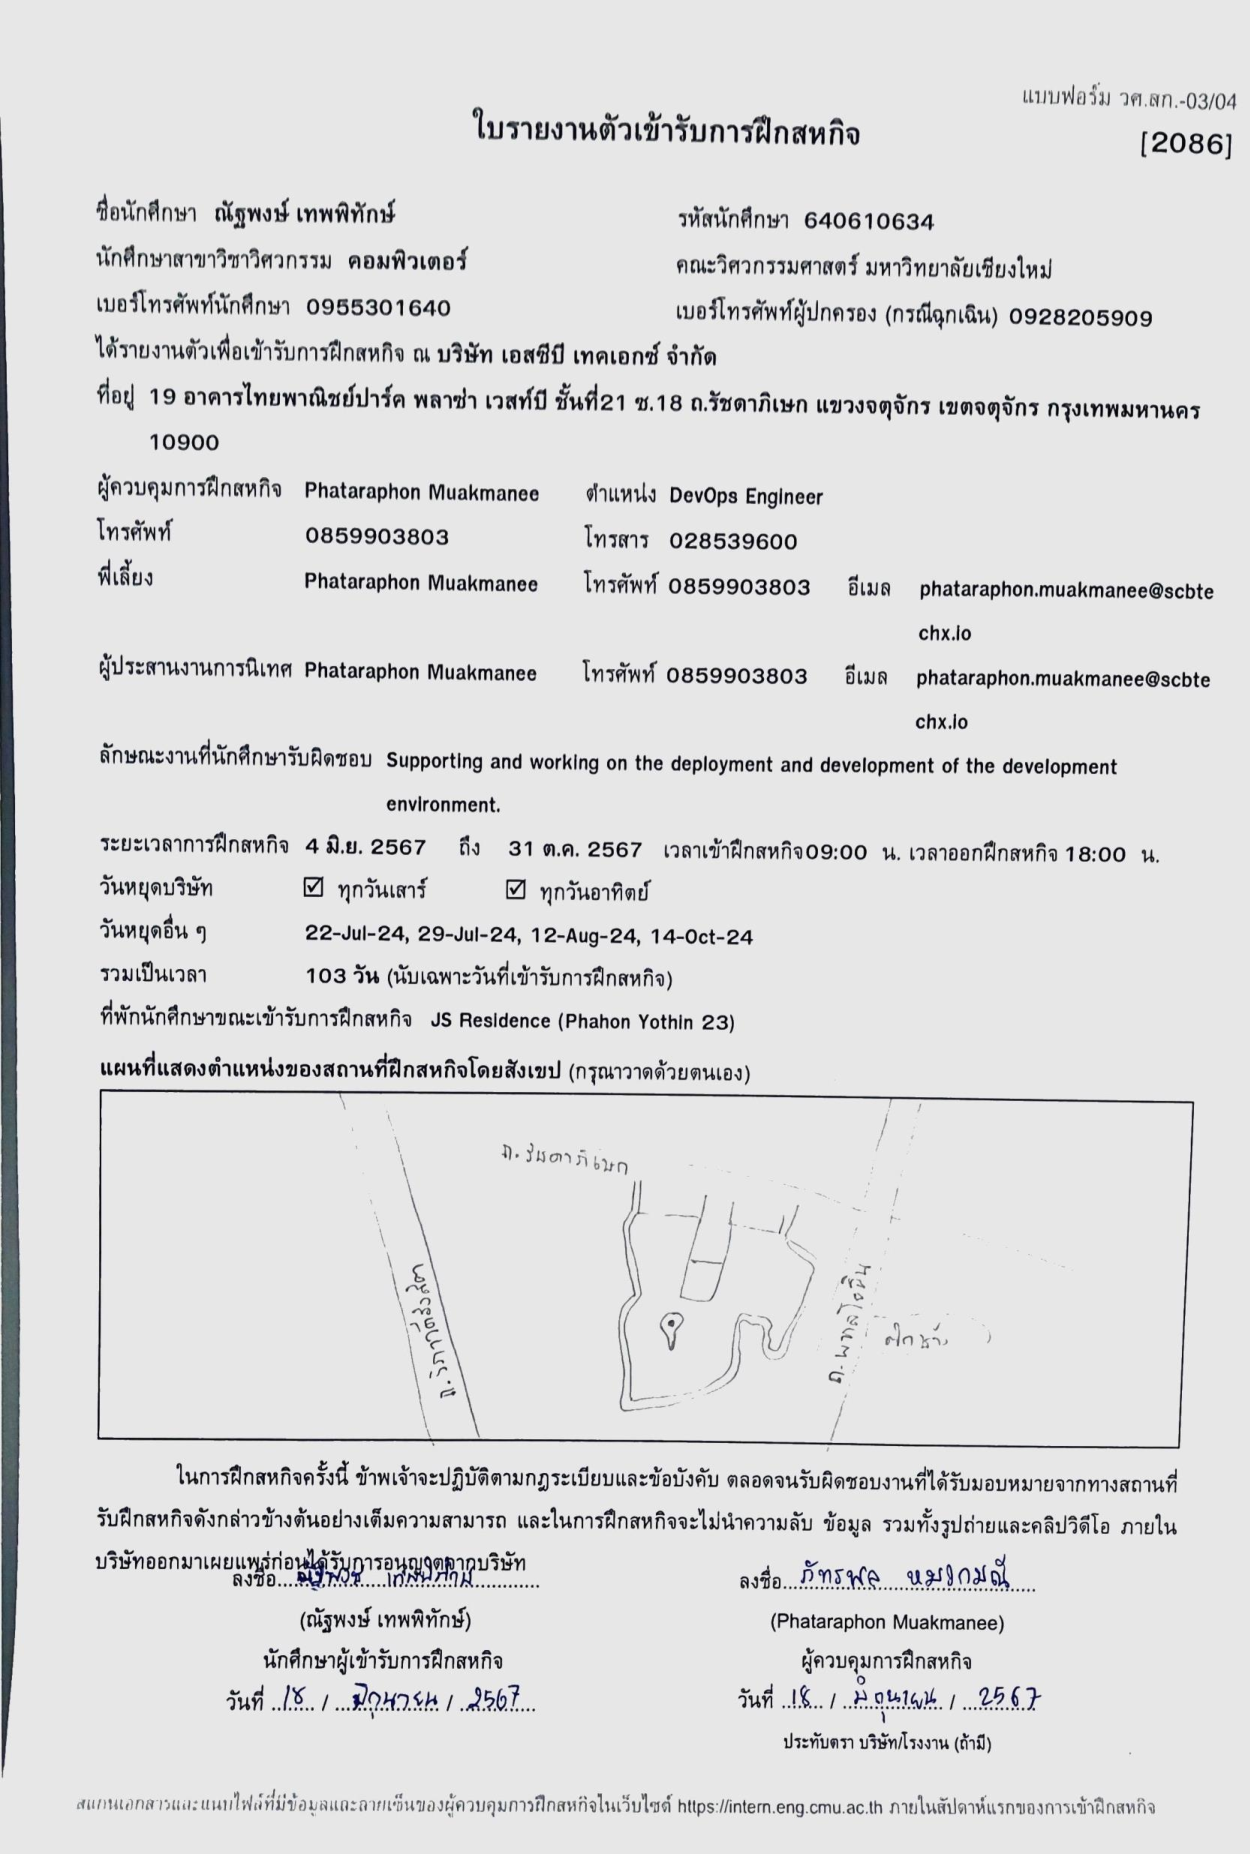
\includepdf[pages=-, scale=.8, pagecommand={\hypertarget{target:03-04}{},\label{page:03-04}}, nup=1x1, frame=true]{pdf/03-04}
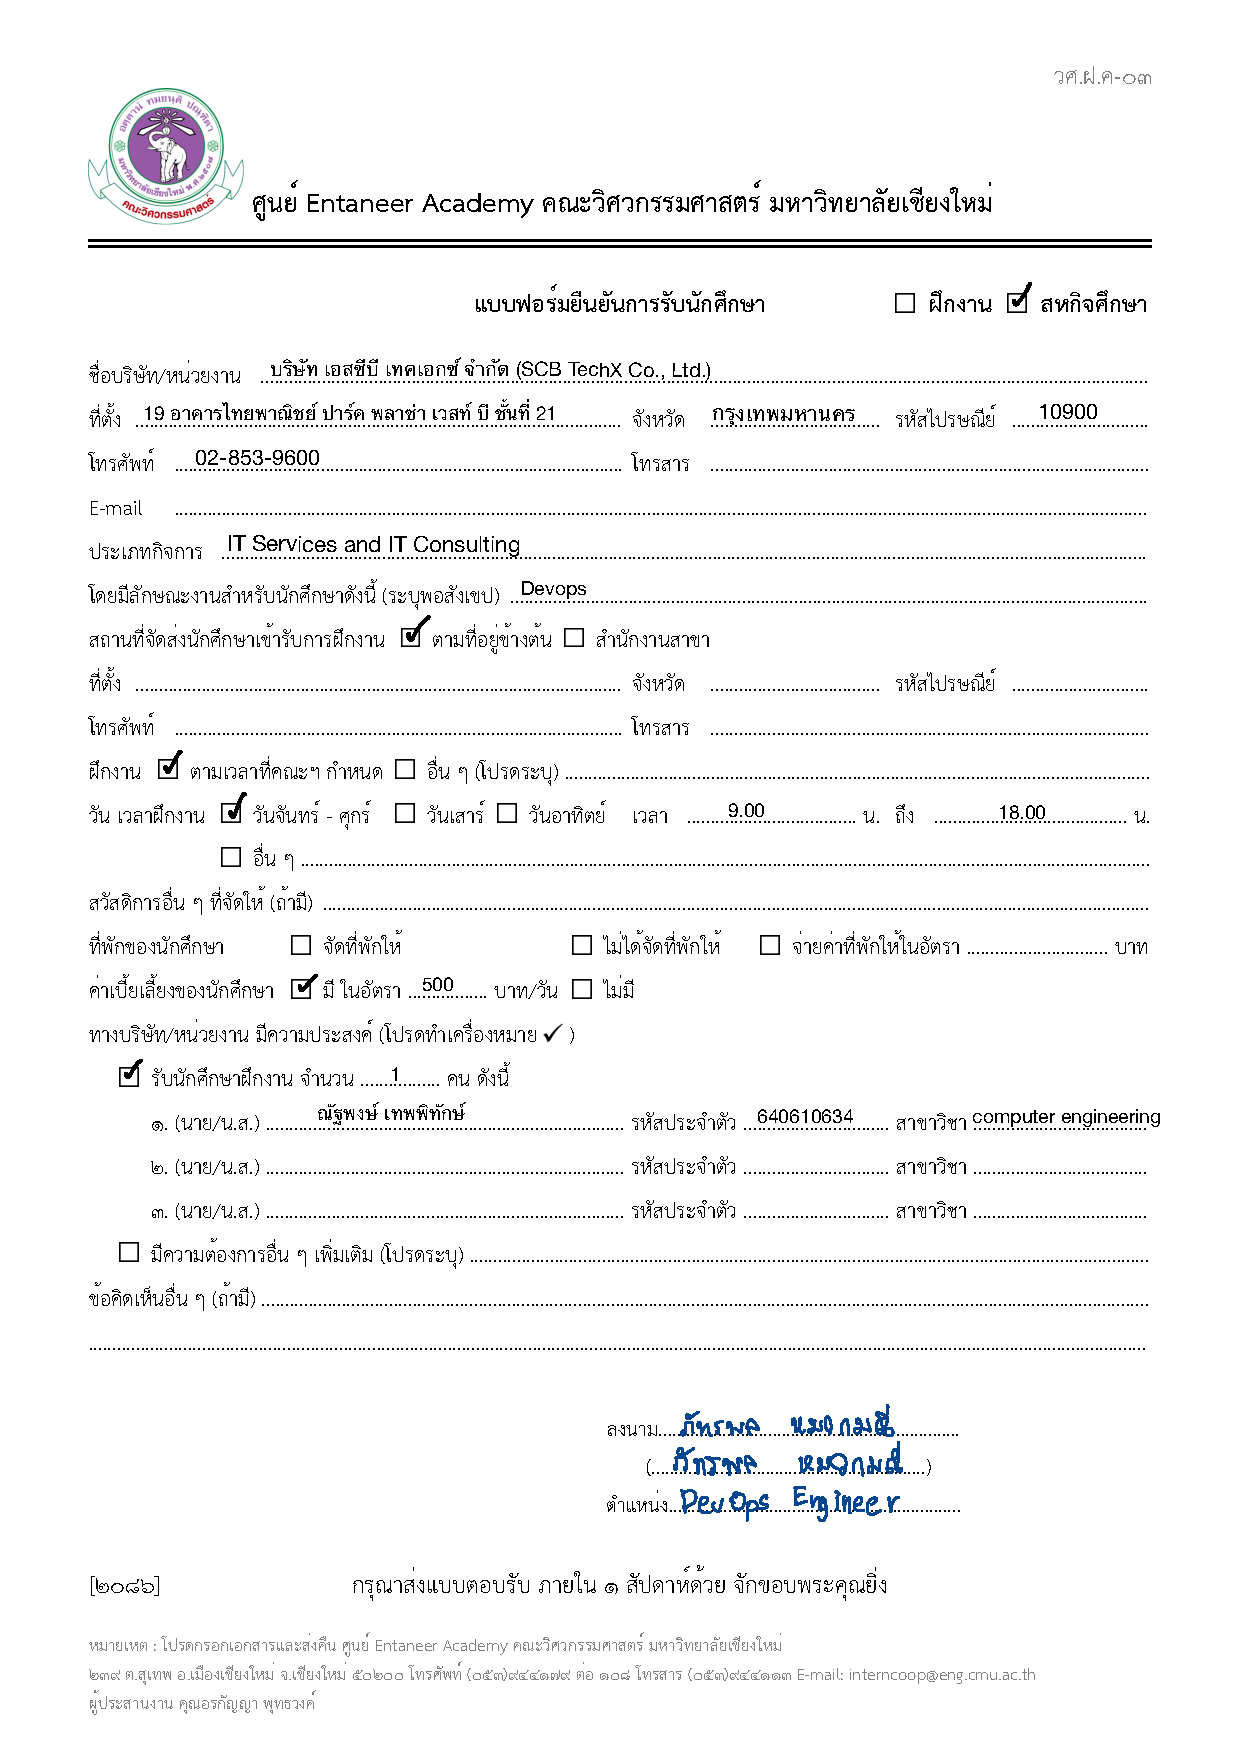
\includepdf[pages=-, scale=.8, pagecommand={\hypertarget{target:03}{},\label{page:03}}, nup=1x1, frame=true]{pdf/03}
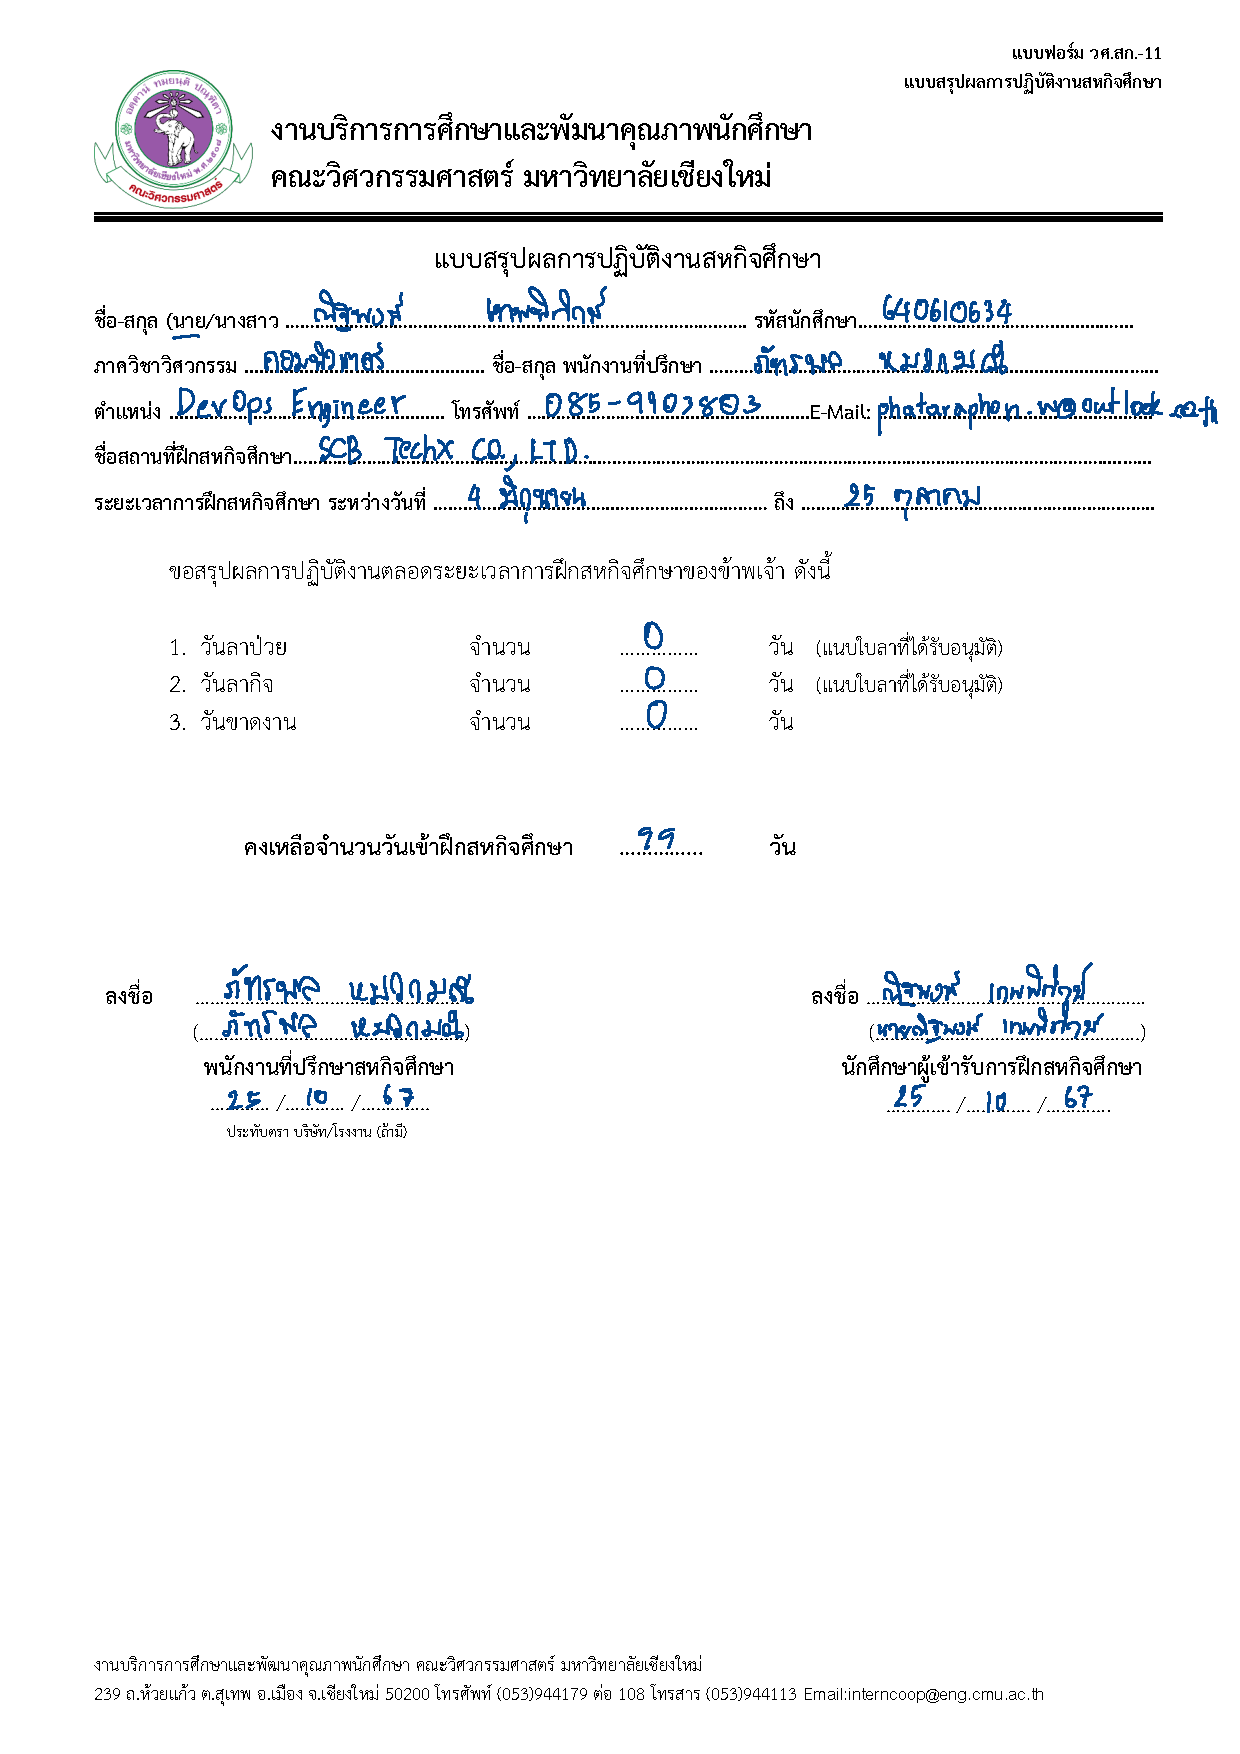
\includepdf[pages=-, scale=.8, pagecommand={\hypertarget{target:11}{},\label{page:11}}, nup=1x1, frame=true]{pdf/11}

% ส่วนที่เกี่ยวข้อง
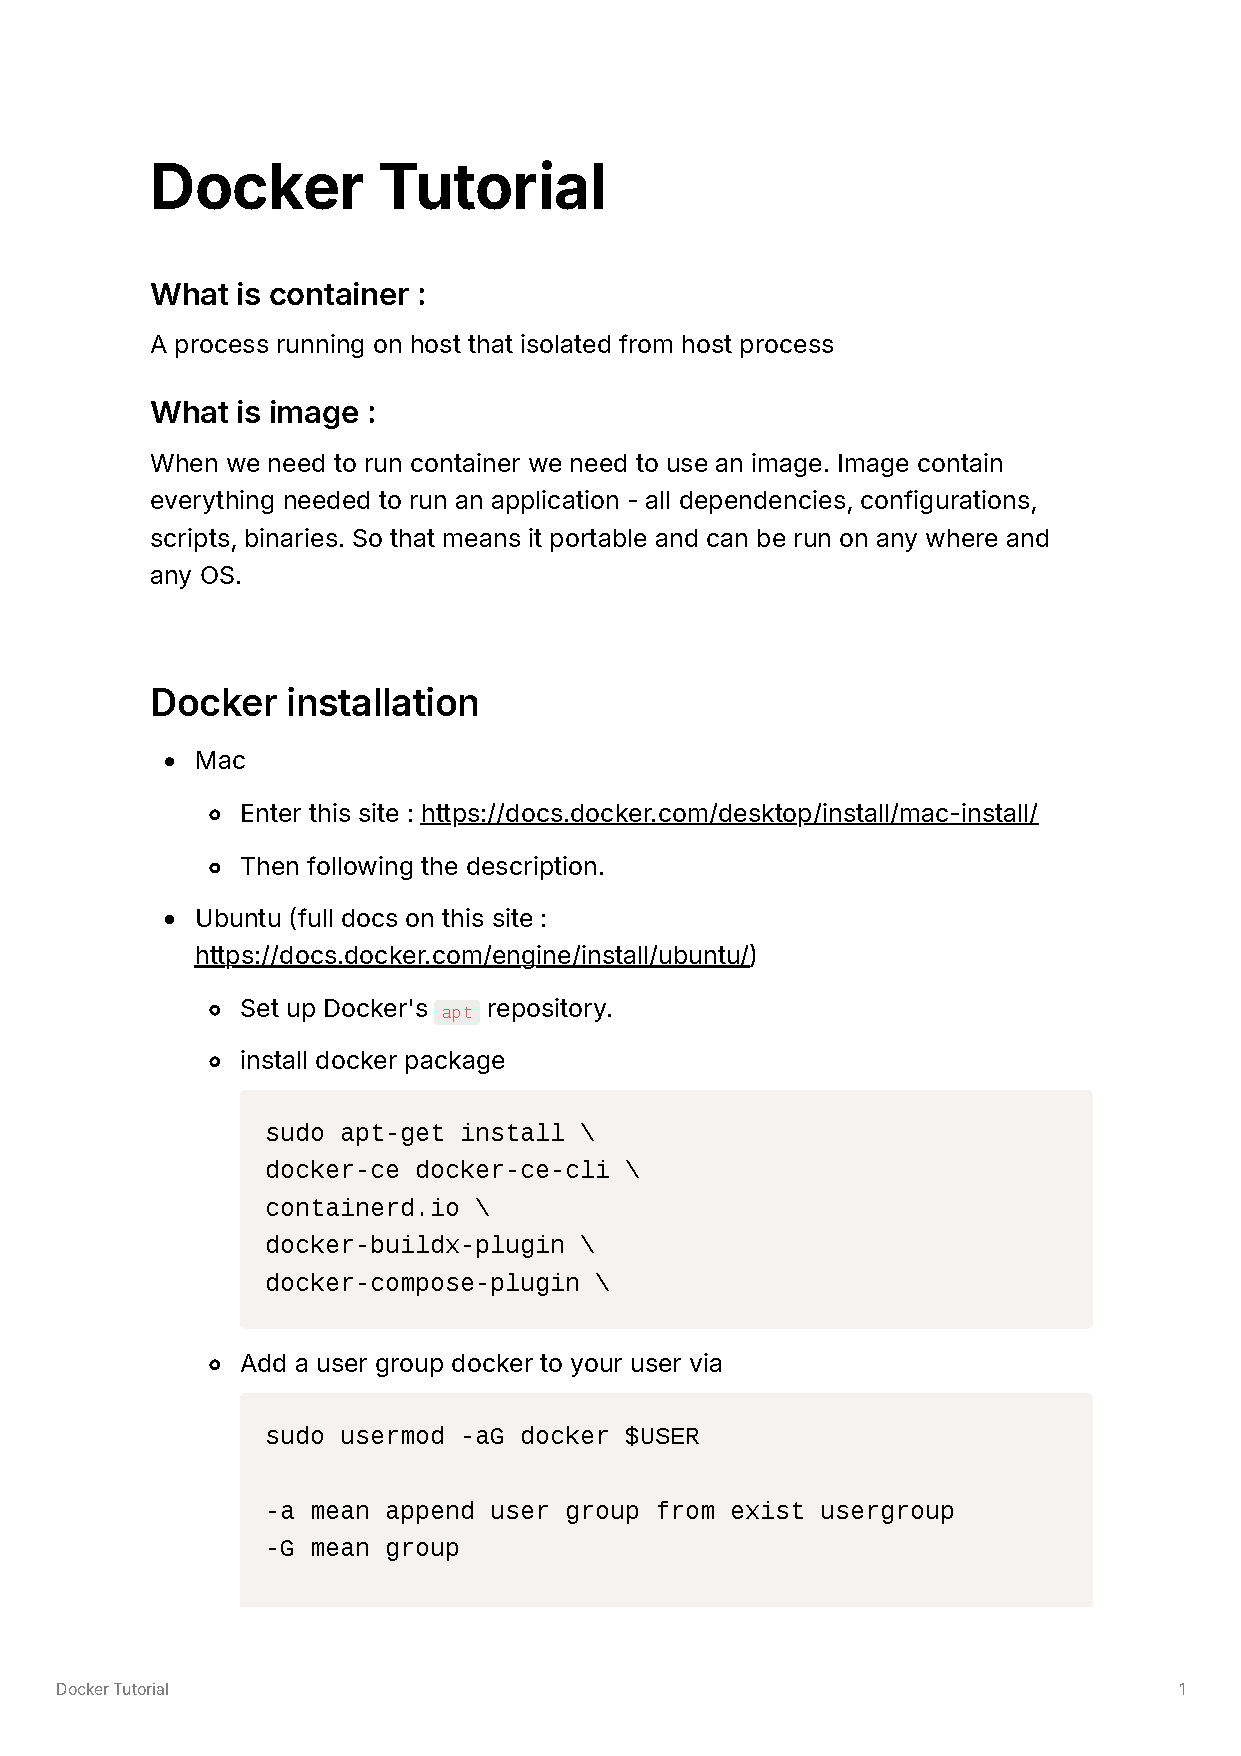
\includepdf[pages=-, scale=.8, pagecommand={\hypertarget{target:docker}{},\label{page:docker}}, nup=1x1, frame=true]{pdf/docker}
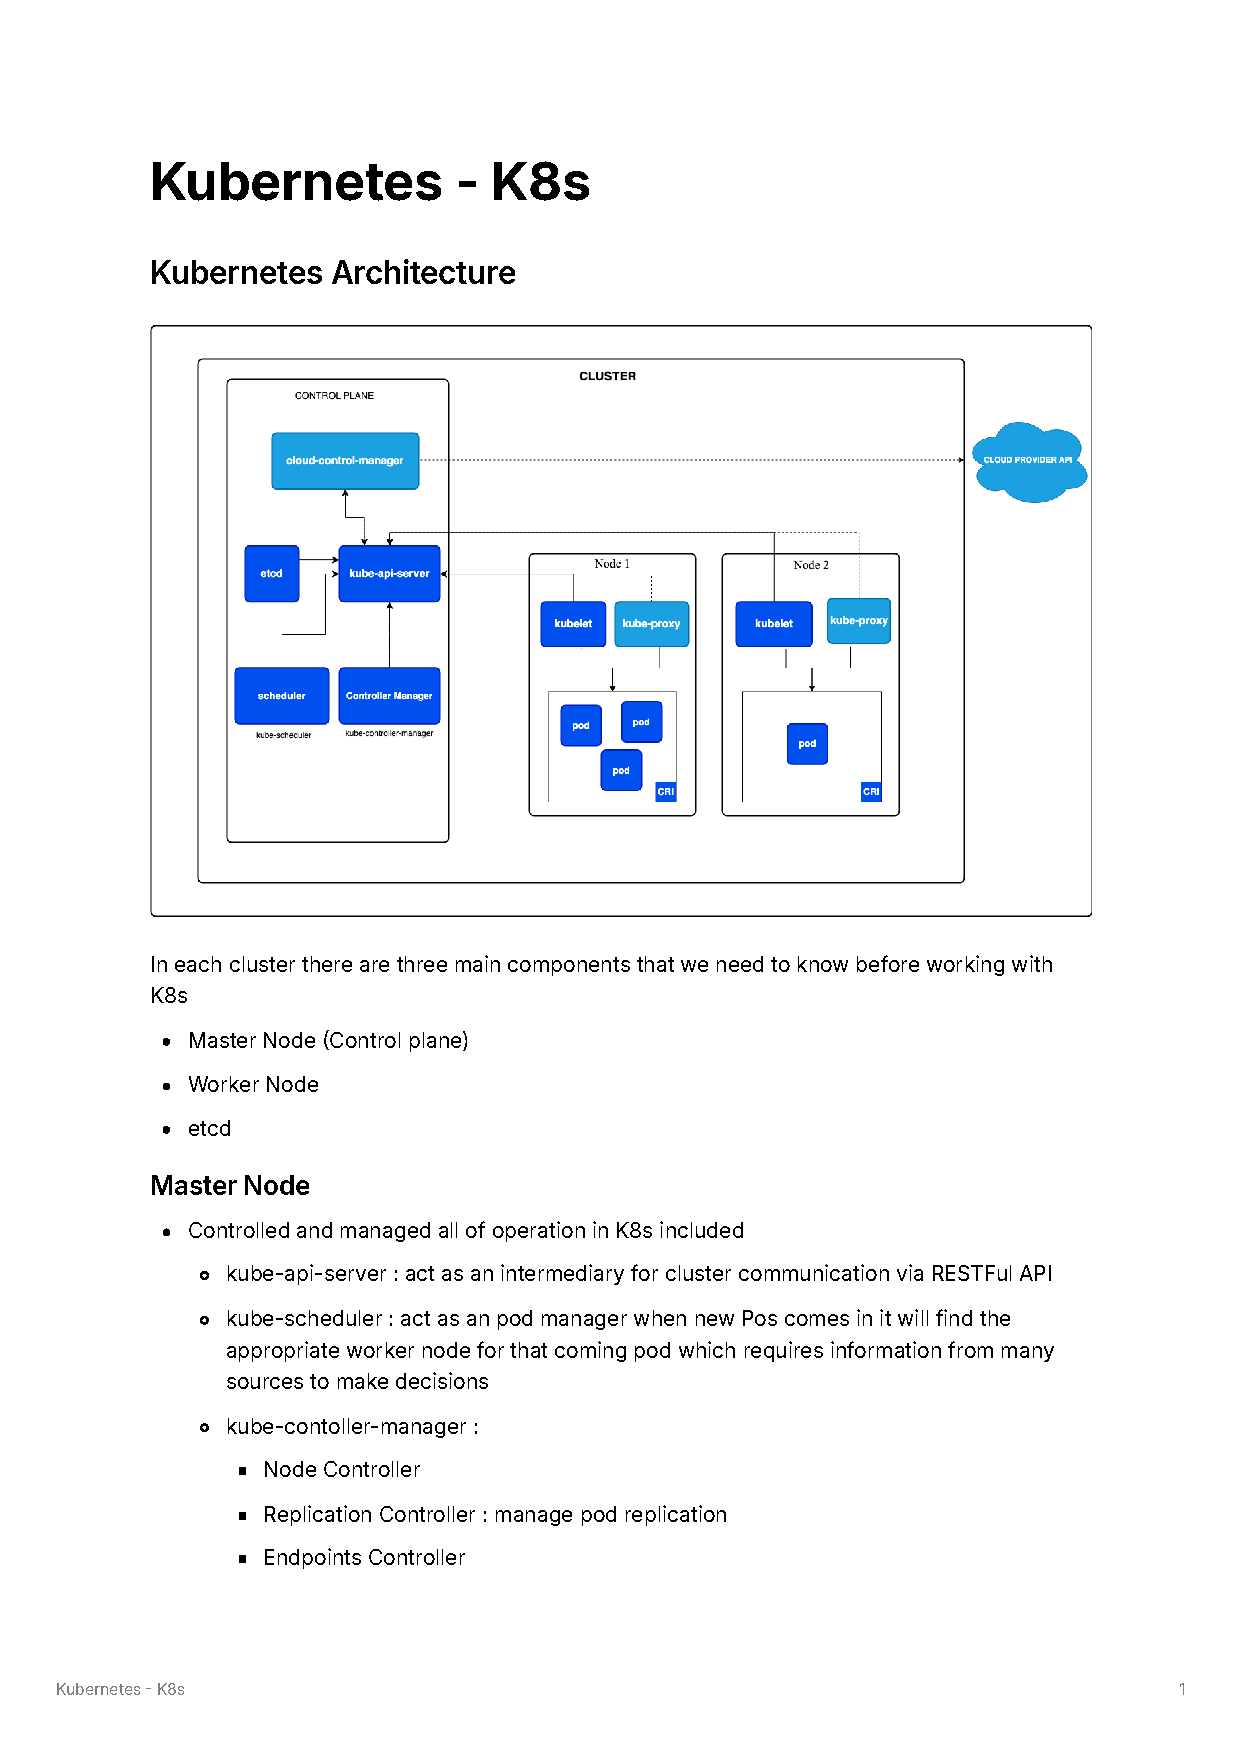
\includepdf[pages=-, scale=.8, pagecommand={\hypertarget{target:kube}{},\label{page:kube}}, nup=1x1, frame=true]{pdf/kube}
\includepdf[pages=-, scale=.8, pagecommand={\hypertarget{target:jenkins}{},\label{page:jenkins}}, nup=1x1, frame=true]{pdf/jenkins}
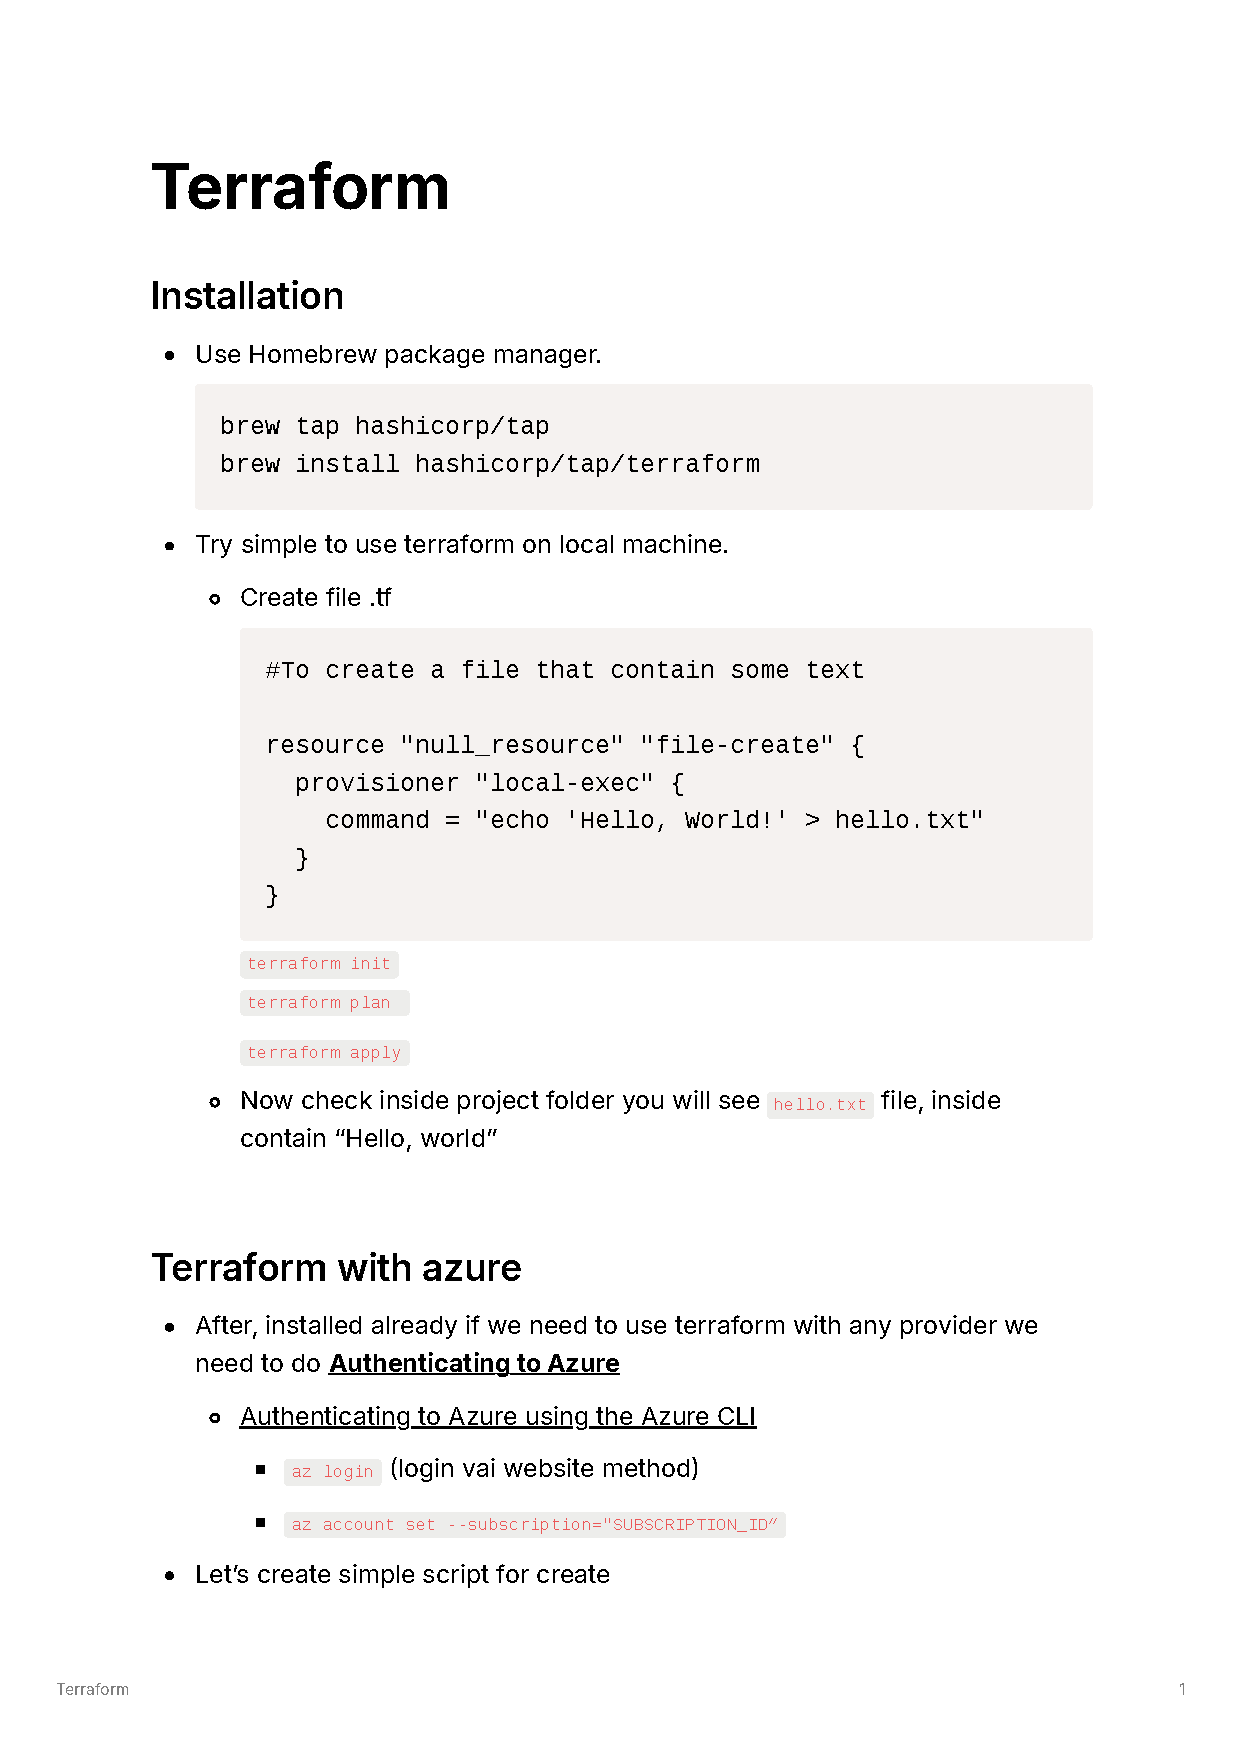
\includepdf[pages=-, scale=.8, pagecommand={\hypertarget{target:terraform}{},\label{page:terraform}}, nup=1x1, frame=true]{pdf/terraform}
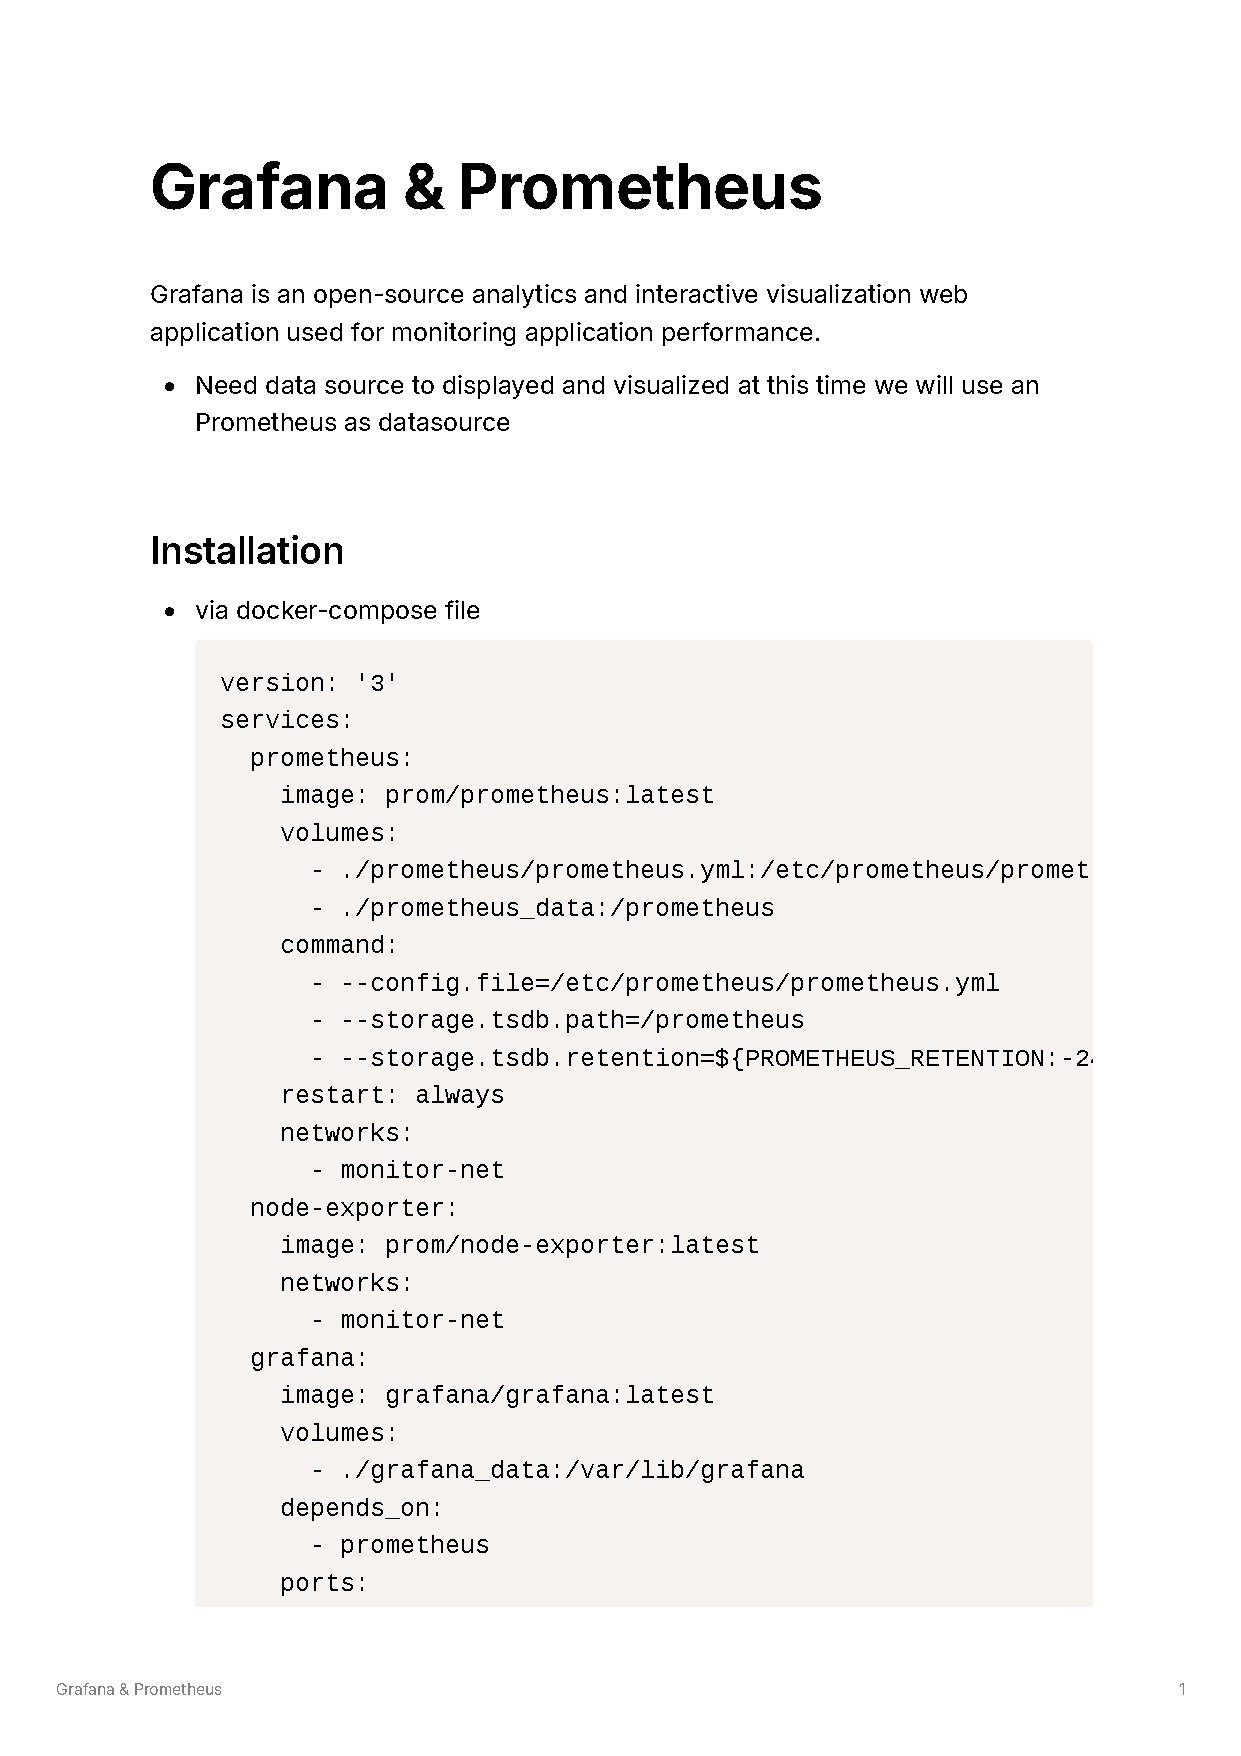
\includepdf[pages=-, scale=.8, pagecommand={\hypertarget{target:monitoring}{},\label{page:monitoring}}, nup=1x1, frame=true]{pdf/monitoring}
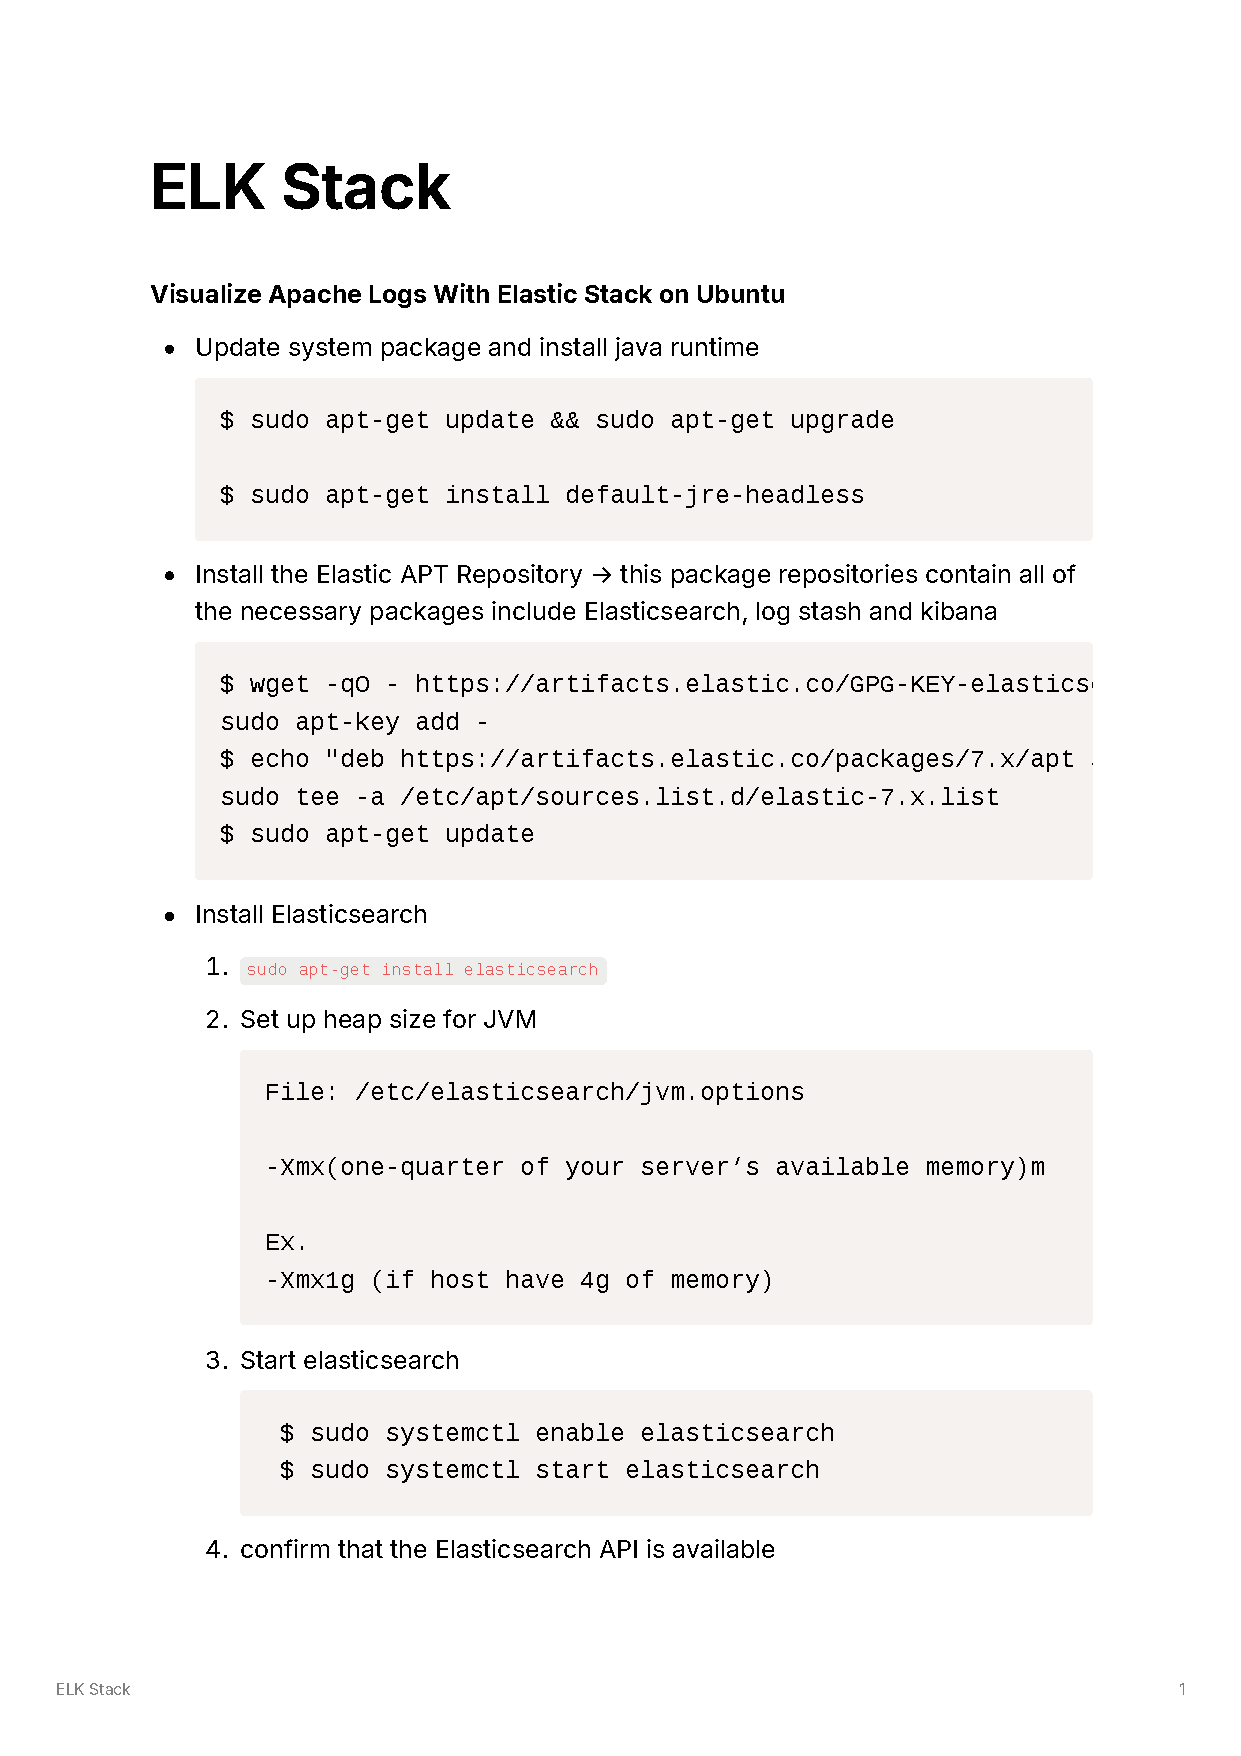
\includepdf[pages=-, scale=.8, pagecommand={\hypertarget{target:elk}{},\label{page:elk}}, nup=1x1, frame=true]{pdf/elk}

%% Display glossary (optional) -- need glossary option.
\ifglossary\glossarypage\fi

%% Display index (optional) -- need idx option.
\ifindex\indexpage\fi

\begin{biosketch}
\begin{center}
  \includegraphics[width=1.5in]{mugshot.jpg}
\end{center}
Your biosketch goes here. Make sure it sits inside
the \texttt{biosketch} environment.
\end{biosketch}
\fi % \ifproject
\end{document}
